\section{Implementation}
\label{sec:implementation}
In the following relevant implementation details will be discussed for each of the main parts of the system. 

The software is to be written using the C programming language. This choice is made based on the familiarity with the language and freedom it provides. Using this language makes the transition into a real world scenario with an embedded platform as the heart of the sensor rather trivial. 
\subsection{Sensor node with dual roles}
\label{subsec:sensornodedesign}
The dual role functionality requires threads, with each thread to handle a particular task these threads are described in Figure \ref{fig:sensorthreads}. One main thread spawns the other threads and is left out. With this structure a node can take two roles - both collecting temperature data and send it to the admin, and receiving data as an admin and process it. Thus sending data to itself as needed.

\begin{figure}[ht!]
\centering
    \begin{subfigure}[b]{0.3\textwidth}
        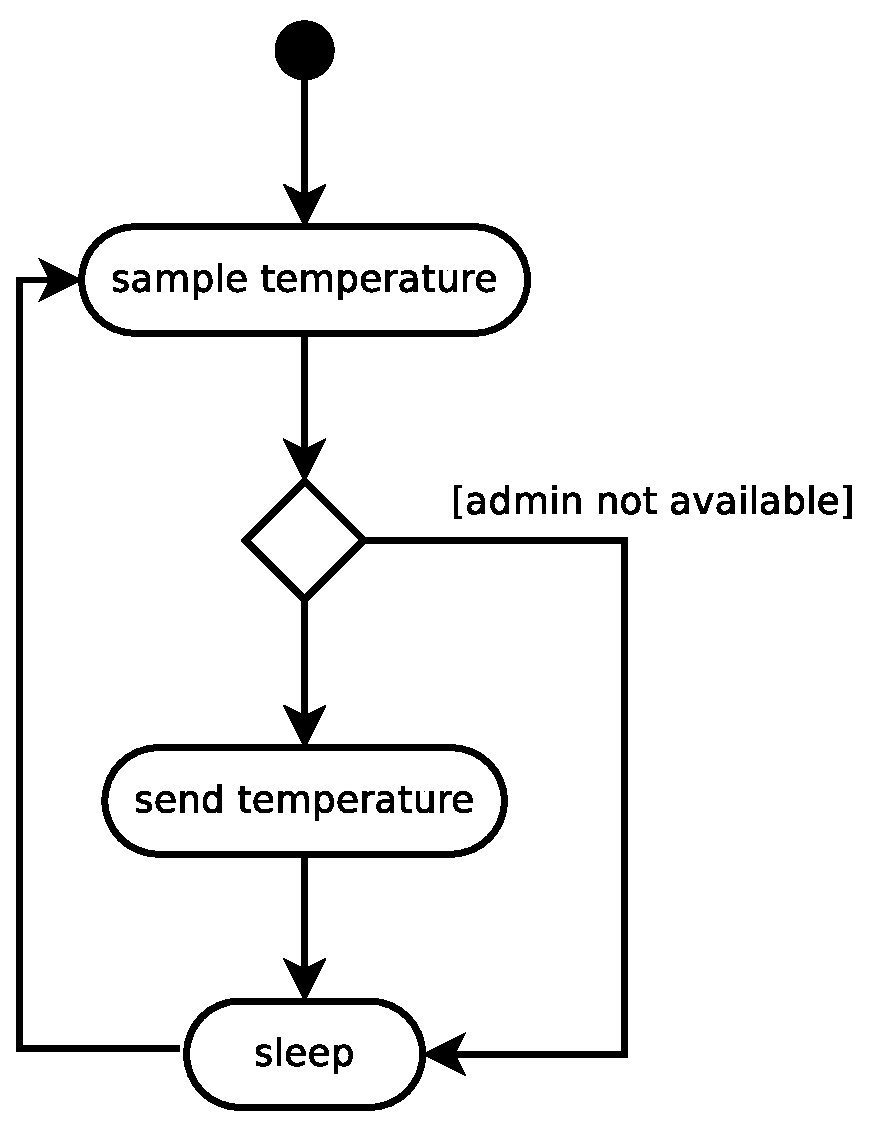
\includegraphics[scale=0.35]{eps/temp_th}
        \caption{Temperature thread}
        \label{fig:tempthread}
    \end{subfigure}
    \begin{subfigure}[b]{0.3\textwidth}
        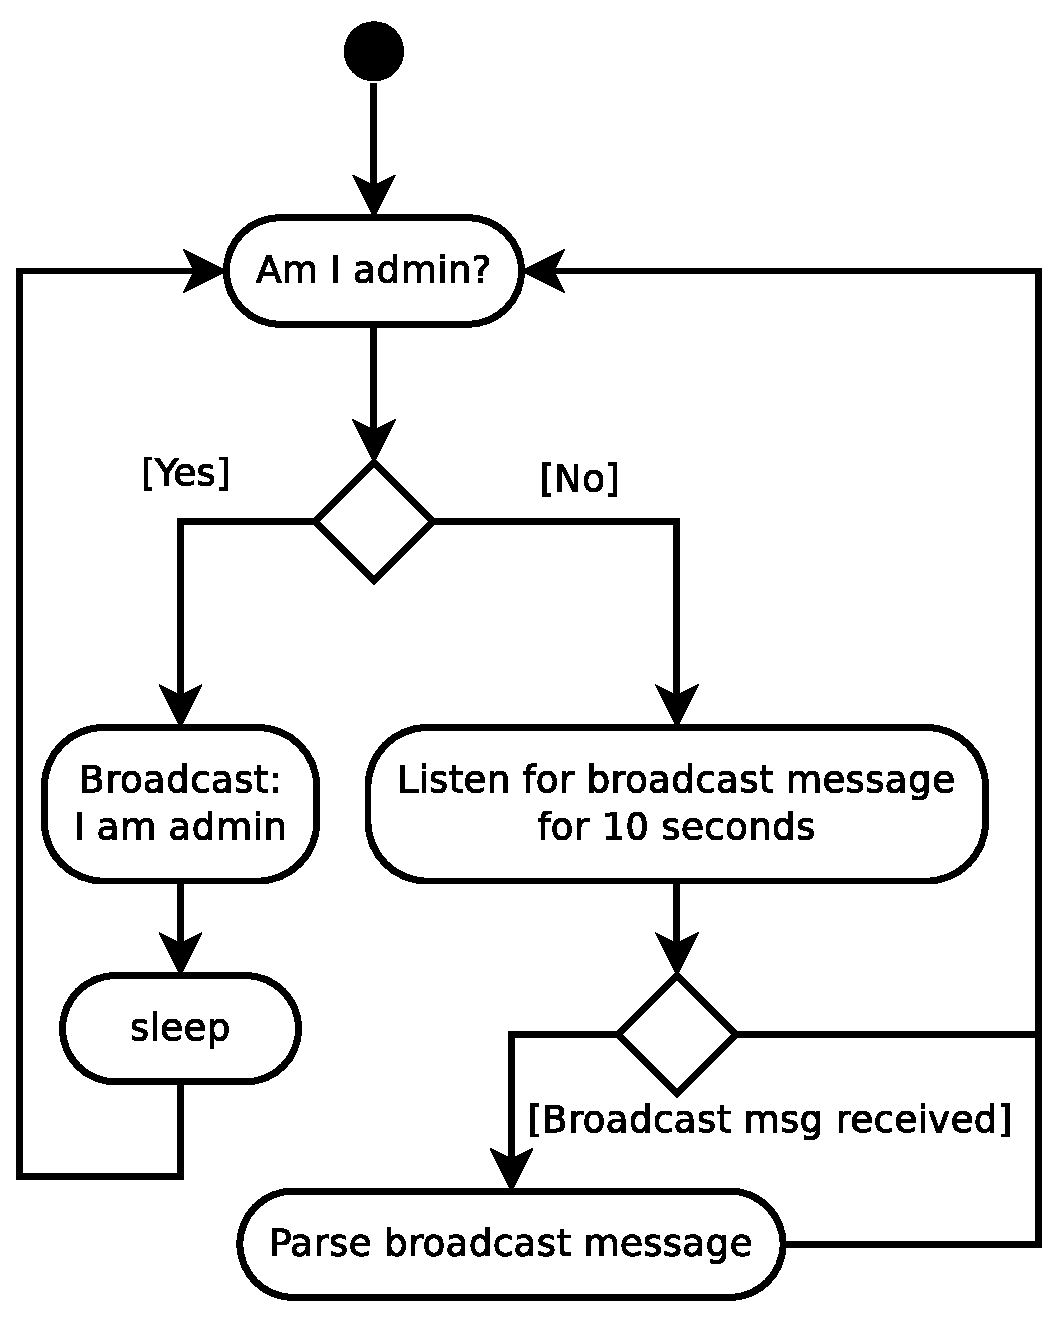
\includegraphics[scale=0.35]{eps/admin_th}
        \caption{Administrator thread}
        \label{fig:adminthread}
    \end{subfigure}
    \qquad
    \begin{subfigure}[b]{0.3\textwidth}
        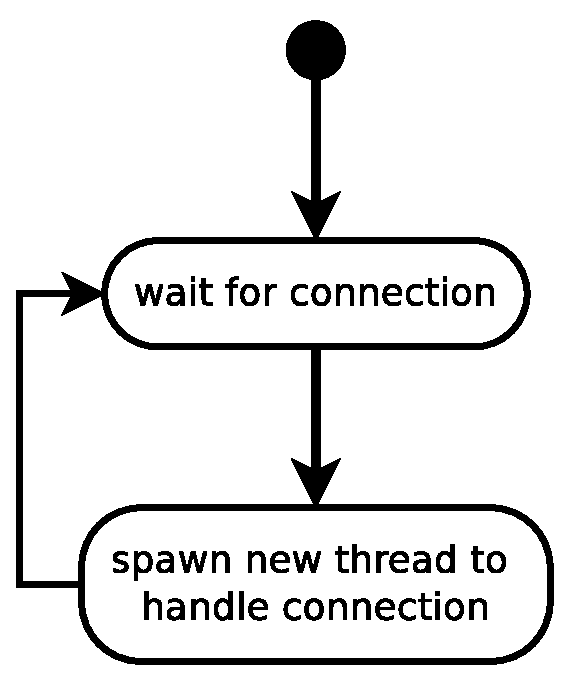
\includegraphics[scale=0.35]{eps/data_th}
        \caption{Data handler thread}
        \label{fig:datathread}
    \end{subfigure}
    \caption{Flow charts on each thread in the sensor}
    \label{fig:sensorthreads}
\end{figure}

\subsection{User entity}
\label{subsec:userdesign}
The user piece of software is a straight forward command line tool. Listing the available options with numbers provides the user with a way to interact with it. Interaction is done by entering a number corresponding to the function and pressing the return key. Main functions are:
\begin{enumerate}
    \item \textbf{Quit:} Ends the program.
    \item \textbf{Connect to node:} Asks for an IP address and opens a connection to that IP.
    \item \textbf{Promote to Admin node:} Initiates the promotion process on the selected node. The admin node is provided a key, that is unique to the admin.
    \item \textbf{Get average T from node:} Requests the average temperature from the available data on the admin node.
\end{enumerate}
The main structure of this program is a simple while()-loop that prints out the menu-options and waits for input on \textit{stdin}. When an input is provided, a switch case evaluates the input and acts accordingly.

\subsection{Message Passing}
\label{subsec:msgpassing}
To transfer messages between the node IP protocol is used. On top of IP protocol, TCP and UDP protocols are used for connection management. TCP protocol is used to provide reliable message passing between user and nodes in the system and between nodes themselves. UDP protocol is used to provide broadcast communications. Due to the fact that UDP protocol does not guarantee delivery of messages, broadcast messages are repeated at set time intervals. UDP broadcast solutions was chosen due to the simplicity of implementation.

\subsection{IP Version agnosticism}
\label{subsec:ipveragn}
Implementation of the sensor system is mostly IP version agnostic. It was implemented this way due to the fact that networks are transitioning from the usage of IP version 4 to IP version 6 protocol. Converting the system to be fully compliant with IP version 6 would require minimal changes in source code. The only change that has to be done is to change the IP address that is used for broadcasting. At the moment broadcasts are sent to the local broadcast address. This broadcasting method is not supported in IP version 6. In IPv6 native systems, broadcast messages should be sent to FF02:0:0:0:0:0:0:1 address which is reserved for multicast ``All nodes address'' communication. Decision to leave IP version 4 method of communication was done mainly due to the fact that IPv4 systems were used for testing.

\subsection{Messages format}
\label{subsec:msgformat}
To provide a scalable solution for message passing, Type-Length-Value (TLV) messages format was used. In TLV messages, each message is encoded in a tuple \{Type, Length, Value\}. Type and Length are integers, first one indicating what kind of message it is and second how long is the Value. TLV encoded messages are easy to serialize and deserialize for sending and later can be easily parsed as a linked list, because all types are known beforehand and length of each message is 2 times length of integer plus value of Length integer. If new message type has to be added, it is enough to add new Type value and update message parsing code with new message type. Serialization, deserialization and parsing code is same regardless of place where it is used - user node, sensor node or master node.  

\subsection{Time offset calculation}
\label{subsec:timesync}
It is assumed in the system model used, that the communication channels are asynchronous. In temperature monitoring system this means that temperature value read in one node can take arbitrary time to reach master node. To solve this issue, time offset calculation is done. When node learns about new master node, it calculates the time offset from node local clock to the master local clock. This time offset then is used to adjust the local timestamp when reporting time when temperature reading was done to the master node. Further more, because all temperature values are timestamped with admin local time, it is easy for admin node to discard old messages. Time offset calculation is done using Network Time Protocol on-wire protocol \cite{ntpv4_standard}. Ilustration of this protocol is provided in Figure~\ref{fig:timeoffset}
\begin{figure}[ht!]
\centering
    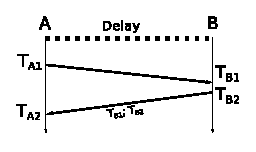
\includegraphics[scale=1]{eps/NTP_onwire_diagram}
\caption{Offset calculation protocol}
\label{fig:timeoffset}
\end{figure}

Protocol operation starts when peer A sends packet at time $T_{A1}$ to peer B. Upon reception of this packet, node creates timestamp when packet was received $T_{B1}$. Then it constructs the reply packet. Receive timestamp is time when packet was received at a server $T_{B1}$. Finally transmit timestamp $T_{B2}$ is added just before sending packet back to peer A. Upon reception of this reply message, peer A creates a timestamp $T_{A2}$ to indicate when packet was received. At this point peer A will calculate offset 

$\theta=\frac{(T_{B1}-T_{A1})+(T_{B2}-T_{A2})}{2}$

This offset is later used to adjust local timestamp when sending messages to master node.

\subsection{Threading}
\label{subsec:threading}
Temperature sensors in this project are implemented using POSIX-threading (Pthreads). Pthreads are used to provide logical separation of tasks in each node. There are separate threads for data messages handling, temperature handling and broadcast messages handling. Using pthreads allowed to achieve error separation (error in one thread logic, will not affect other thread) and also easier workload distribution between programmers. Second place where pthreads are used is handling of multiple connections. Many application written in C use fork() system call to handle connection, but this was not an option for this implementation, because of the need of global variables visible from all threads.
\label{subsec:msgpass}
